\documentclass{beamer}

\usepackage{fontspec}
\usepackage[utf8]{inputenc}
\usepackage[cache=false]{minted}
\usepackage{hyperref}
\usepackage{graphicx}

\usetheme{Madrid}
\setmonofont{Fira Code}
\newmintedfile[haskellcode]{haskell}{style=trac}
\newmintedfile[shelllog]{console}{style=murphy}
\definecolor{shellcolor}{gray}{0.6}
\newcommand{\inlinehaskell}[1]{\mintinline[style=trac]{haskell}{#1}}
\newcommand{\inlineshell}[1]{\textcolor{shellcolor}{\textbf{#1}}}
\hypersetup{colorlinks=false}
\AtBeginSection[]
{
  \begin{frame}
    \frametitle{Contents}
    \tableofcontents[currentsection]
  \end{frame}
}
%--------------------------------------------

\title[Laziness in GHC Haskell]
{Laziness in GHC Haskell}

\subtitle{The features and principles}

\author[chip]
{Presented by chip}

\institute[ZJU]
{
  ZJU Lambda\\
  From here to World
}

\date[ZJU-Lambda 2019]
{ZJU-Lambda Conference, May 2019}

\logo{
\includegraphics[height=1.2cm]{./pic/haskell-logo.png}}

\begin{document}
\frame{\titlepage}


\section{Appetizers}
%--------------------------------------------

\begin{frame}
\frametitle{Course 1: Outside in}
\haskellcode{src/outside-in.hs}
\par\noindent\rule{0.75\textwidth}{1.0pt}
\newline\newline
If we apply \inlinehaskell{possiblyBottom} to \inlinehaskell{True}, we will get a \inlinehaskell{0}.
\end{frame}

%--------------------------------------------

\begin{frame}
\frametitle{Course 1: Outside in}
A slightly arcane form:\newline
\haskellcode{src/arcane-form.hs}
\end{frame}

%--------------------------------------------

\begin{frame}
\frametitle{Course 1: Outside in}
Nesting lambdas and reducing from the outside in:\newline
(They are not in fact decomposed this way by the compiler)\newline
\haskellcode{src/lambda-nesting.hs}
\end{frame}

%--------------------------------------------

\begin{frame}
\frametitle{Course 2: Evaluate to WHNF}
\haskellcode{src/evaluate-to-WHNF.hs}
\par\noindent\rule{0.7\textwidth}{1.0pt}
\newline\newline
It prints \inlinehaskell{2} !
\newline
What happened here?
\end{frame}

%--------------------------------------------

\begin{frame}
\frametitle{Example 2: Evaluate to WHNF}
The actual evaluation process:
\newline
\haskellcode{src/length'-procedure.hs}
\begin{block}{Concept}
In WHNF, we only evaluate the outermost constructor
\end{block}
\end{frame}


\section{Thunk? What's it?}
%--------------------------------------------

\begin{frame}
\frametitle{The Haskell Heap}
\begin{center}
    The Haskell heap is a rather strange place.
\end{center}
\begin{figure}[hbt!]
    \centering
    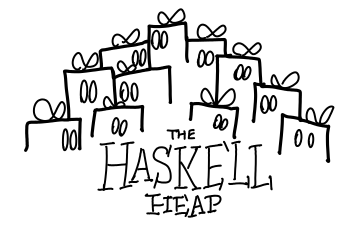
\includegraphics[height=0.5\textheight]{./pic/haskell-heap.png}
\end{figure}
\end{frame}

%--------------------------------------------

\begin{frame}
\frametitle{Box}
Every item is wrapped up nicely in a box:\newline
The Haskell heap is a heap of \textit{presents} (thunks).
\begin{figure}[hbt!]
    \centering
    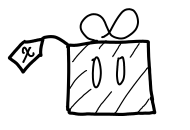
\includegraphics[height=0.4\textheight]{./pic/thunk.png}
\end{figure}
\end{frame}

%--------------------------------------------

\begin{frame}
\frametitle{Present}
When you actually want what’s inside the present, you \textit{open it up} (evaluate it).\newline
\begin{figure}[hbt!]
    \centering
    
\includegraphics[height=0.4\textheight]{./pic/thunk-nullary.png}
\end{figure}
\end{frame}

%--------------------------------------------

\begin{frame}
\frametitle{Gift card}
Sometimes you open a present, you get a \textit{gift card} (data constructor).\newline
Gift cards have two traits.\newline
\begin{itemize}
    \item A name. (the \textbf{Just} gift card or \textbf{Right} gift card)\newline
    \item And they tell you where the rest of your presents are.\newline
\end{itemize}
There might be more than one (the tuple gift card), if you’re a lucky duck!
\begin{figure}[hbt!]
    \centering
    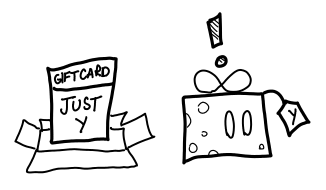
\includegraphics[height=0.4\textheight]{./pic/thunk-constructor.png}
\end{figure}
\end{frame}

%--------------------------------------------

\begin{frame}
\frametitle{Tricksters}
Presents on the Haskell heap are rather mischievous.\newline

\begin{columns}
\column{0.5\textwidth}
\begin{figure}[hbt!]
    
\includegraphics[height=0.3\textheight]{./pic/thunk-bomb.png}
\end{figure}
\begin{center}
Explode when you open it
\end{center}

\column{0.5\textwidth}
\begin{figure}[hbt!]
    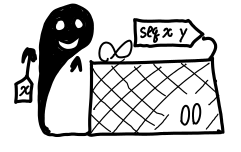
\includegraphics[height=0.3\textheight]{./pic/thunk-ghost.png}
\end{figure}
\begin{center}
Haunted by ghosts that open other presents when disturbed
\end{center}
\end{columns}
\end{frame}

%--------------------------------------------

\begin{frame}
\frametitle{What is a \textit{thunk}?}
\inlinehaskell{<thunk: expression-to-be-evaluated>}
\begin{itemize}
    \item A box containing unevaluated expressions.
    \item Being evaluated when \textit{needed}.
    \item Basically \textbf{anything} creates a thunk in (GHC) Haskell, by default
\end{itemize}

\begin{figure}[hbt!]
\begin{center}
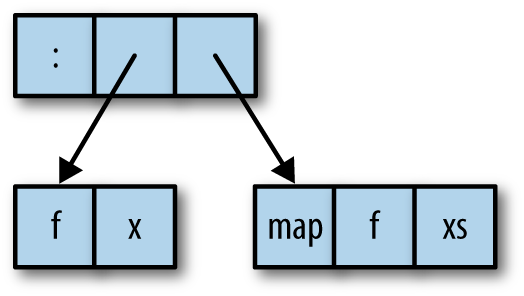
\includegraphics[height=0.4\textheight]{./pic/thunk-map.png}
\caption{Thunks created by a map}
\end{center}
\end{figure}
\end{frame}

%--------------------------------------------

\begin{frame}
\frametitle{Example: Evaluate a thunk}
\haskellcode{./src/thunk-sprint.hs}
\begin{block}{Important}
Once evaluated, the thunk is replaced by its \textit{actual} value.
\end{block}
\end{frame}

%--------------------------------------------

\begin{frame}
\frametitle{Thunk brings us...}
\begin{itemize}
    \item On-demand data types.
    \item Call-by-need strategy.
    \item Result sharing on CAF (Constant Applicative Forms).
    \item ...
\end{itemize}\bigskip
\haskellcode{./src/fibs.hs}
\end{frame}


\section{Why we need strictness?}
%--------------------------------------------

\begin{frame}
\frametitle{Thunks are good, but...}
\haskellcode{src/lazy-foldl.hs}\bigskip
What about \inlinehaskell{foldl (+) 0 [1..1000000000]} ?\newline
\begin{figure}[hbt!]
    \centering
    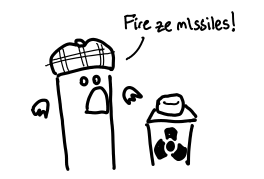
\includegraphics[height=0.4\textheight]{./pic/evil-of-thunk.png}
\end{figure}
\end{frame}

%--------------------------------------------

\begin{frame}
\frametitle{Memory leak}
After executing \inlinehaskell{foldl (+) 0 [1..1000000000]}\newline
\begin{figure}[hbt!]
    \centering
    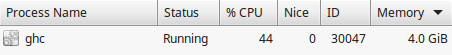
\includegraphics[height=0.1\textheight]{./pic/memory-usage-ghc.png}
    \newline\newline
    A veritable ghost jamboree in our memory!
    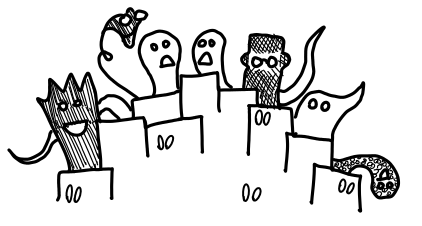
\includegraphics[height=0.4\textheight]{./pic/ghost-party.png}
\end{figure}
\end{frame}

%--------------------------------------------

\begin{frame}
\frametitle{RTS - a non-trivial Runtime System}
\begin{figure}[hbt!]
\begin{center}
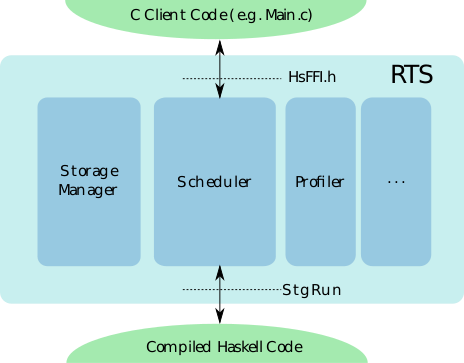
\includegraphics[height=0.6\textheight]{./pic/rts-overview.png}
\caption{RTS Overview}
\end{center}
\end{figure}
\end{frame}

%--------------------------------------------

\begin{frame}
\frametitle{Example: Profiling}
\haskellcode{src/profiling.hs}
\end{frame}

%--------------------------------------------

\begin{frame}
\frametitle{Statistics}
Compile it.\newline
\inlineshell{ghc --make -rtsopts -O2 a.hs}\newline
\inlineshell{./a 1e7 +RTS -sstderr}\newline\newline
Output:\newline
\shelllog{./src/profiling.stderr}
\end{frame}

%--------------------------------------------

\begin{frame}
\frametitle{Basic Profiling}
Mark the cost centres
\begin{itemize}
    \item SCC pragma
    \item Option \inlineshell{-auto-all}
    \item and \inlineshell{-caf-all}, if needed
\end{itemize}\bigskip

Then, compile with option \inlineshell{-prof}\newline
Run \inlineshell{./a 1e7 +RTS -p}, we get a file \inlineshell{a.prof}
\end{frame}

%--------------------------------------------

\begin{frame}
\frametitle{Basic Profiling}
\begin{figure}[hbt!]
\begin{center}
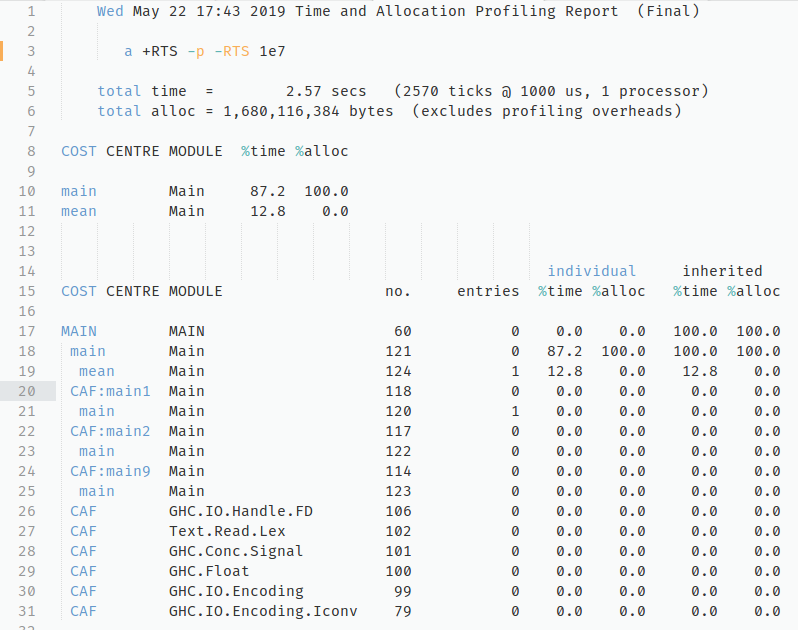
\includegraphics[height=0.7\textheight]{./pic/profiling.png}
\caption{Profiling message generated by RTS}
\end{center}
\end{figure}
\end{frame}

%--------------------------------------------

\begin{frame}
\frametitle{Heap Profiling}

\begin{figure}[hbt!]
\begin{center}
\includegraphics[height=0.7\textheight]{./pic/profiling-hd.ps}
\caption{Break by constr­uct­or/­closure}
\end{center}
\end{figure}
\end{frame}


\section{Optimization}
%--------------------------------------------

\begin{frame}
\frametitle{Example}
Where might be the cost centres?
\newline
\haskellcode{./src/optimization-original.hs}
\end{frame}

%--------------------------------------------

\begin{frame}
\frametitle{Method 1: Using strict functions}
\haskellcode{./src/optimization-strict-fold.hs}
\par\noindent\rule{0.85\textwidth}{1.0pt}
\newline\newline
Why can't we just write \inlinehaskell{(n,s) `seq` (n+1, s+x)} ?
\end{frame}

%--------------------------------------------

\begin{frame}
\frametitle{Method 2: Bang patterns}
\haskellcode{./src/optimization-bang-patterns.hs}
\end{frame}

%--------------------------------------------

\begin{frame}
\frametitle{Method 3: Strict data types}
\haskellcode{./src/optimization-strict-types.hs}
\par\noindent\rule{0.85\textwidth}{1.0pt}
\newline\newline
The \inlinehaskell{Pair} will always store its fields in WHNF.
\end{frame}

%--------------------------------------------

\begin{frame}
\frametitle{Method 4: Unbox values}
Introduction: Core
\begin{itemize}
    \item An intermediate language used by GHC.
    \item Resembles a subset of Haskell
    \item Explicit type annotations ($F_C$)
    \item Type equality constraints and safe coercions
\end{itemize}
\bigskip
To check the Core, compile with \inlineshell{-ddump-simpl}
\end{frame}


%--------------------------------------------

\begin{frame}
\frametitle{Method 4: Unbox values}
Simplified Core: inlined \inlinehaskell{fold'}
\newline
\haskellcode{./src/optimization-core-boxed.hs}
\par\noindent\rule{0.8\textwidth}{1.0pt}
\newline\newline
More to optimize?
\end{frame}


%--------------------------------------------

\begin{frame}
\frametitle{Method 4: Unbox values}
Avoid heap checking:
\inlinehaskell{data Pair = Pair !Int !Double}\newline
Unbox the \inlinehaskell{Pair}:
using flag \inlineshell{-funbox-strict-fields}
\newline
\haskellcode{./src/optimization-core-unboxed.hs}
\par\noindent\rule{0.9\textwidth}{1.0pt}
\newline\newline
Now, except the nodes of list, all the values are stored in registers.
\end{frame}

%--------------------------------------------

\begin{frame}
\frametitle{Statistics}
Compile it.\newline
\inlineshell{ghc --make -funbox-strict-fields -rtsopts -O2 a.hs}\newline
\inlineshell{./a 1e7 +RTS -sstderr}\newline\newline
Output:\newline
\shelllog{./src/optimization.stderr}
\end{frame}

%--------------------------------------------

\begin{frame}
\frametitle{Summary}
\begin{tabular}{ccccc}
\hline
    &  Memory used  &   MUT  &      GC        & Total\\
\hline
Original  & 1519 MB & 2.905s & 8.936s(75.3\%) & 11.865s\\
Optimized &   1 MB  & 1.490s & 0.016s(1.0\%) &  1.509s\\
\hline
\end{tabular}
\newline\newline
What we can learn is:
\begin{itemize}
    \item Compile with \inlineshell{-O2} flag.
    \item Go profiling(Time/Heap) when confused.
    \item Avoid calculations piling up (using strictness).
    \item Unbox atom types \inlinehaskell{(Int, Double,...)}
    \item Use types that can be transformed into primitives (\inlinehaskell{Int} instead of \inlinehaskell{Integer})
\end{itemize}
\end{frame}

%--------------------------------------------

\begin{frame}
\frametitle{Further optimization}
\begin{itemize}
    \item Deforestation (remove intermediate structures)
    \item Rely on gcc -O2 (\inlineshell{-fvia-C -optc-O2})
\end{itemize}
\bigskip
In our example, we can use a deforestation called \textbf{stream fusion}.\newline
It turns \textit{recursive list generation} and \textit{transformation functions} into \textit{non-recursive unfolds}
\end{frame}

\begin{frame}
\frametitle{Stream fusion}
\haskellcode{./src/optimization-fusion.hs}
\end{frame}


\section{Tasty seq}
%--------------------------------------------

\begin{frame}
\frametitle{Using \textit{seq}}
\inlinehaskell{seq :: a -> b -> b}\newline
\inlinehaskell{seq} evaluates its first argument to \textbf{WHNF}, and return the second one.\newline

\inlinehaskell{($!) :: (a -> b) -> a -> b  -- |infixr 0|}\newline
\inlinehaskell{$!} is similar with \inlinehaskell{$}, but evaluates its argument to \textbf{WHNF}.
\end{frame}

%--------------------------------------------

\begin{frame}
\frametitle{Control.DeepSeq}
\haskellcode{./src/deepseq.hs}
\end{frame}

%--------------------------------------------

\begin{frame}
\frametitle{Control.Parallel}
\inlinehaskell{par :: a -> b -> b  -- |infixr 0|}\newline
Indicates that it may be beneficial to evaluate the first argument in parallel with the second. Returns the value of the second argument.\newline

\inlinehaskell{pseq :: a -> b -> b   -- |infixr 0|}\newline
Guarantee the order of evaluation in parallelism.\newline
\newline\pause
Possible transformation on \inlinehaskell{seq}:\newline
\inlinehaskell{a `seq` b <==> b `seq` a `seq` b}
\end{frame}

%--------------------------------------------

\begin{frame}
\frametitle{More on parallel programming}
Please refer to:\newline\newline
\textbf{Control.Parallel.Strategies} (deterministic parallelism)\newline\newline
\textbf{Control.Concurrent} (non-deterministic parallelism)\newline\newline
\href{http://simonmar.github.io/bib/papers/strategies.pdf}{Seq no more: Better Strategies for Parallel Haskell}
\end{frame}

%--------------------------------------------

\begin{frame}
\frametitle{Thank you!}
\begin{center}
    This work is licensed under \textbf{CC-BY-SA 4.0}
    \newline
    \href{https://creativecommons.org/licenses/by-sa/4.0/}{Creative Commons Attribution Share Alike 4.0 International}
    \newline\newline
    You can find the slides on my \href{https://github.com/sakamitz/latex-presentations/tree/master/laziness-of-ghc}{\textbf{Github}}
    \newline\newline
    (The hyperlinks really exist, but they are not colored. x)
\end{center}
\end{frame}

\end{document}